Using a Data Requirements document we can construct an ER diagram, take for example the following:
\begin{verbatim}
    Company Data Requirements:
    The company is organized into branches. Each branch has a unique number, a name, and a particular employee who manages it.

    The company makes it's money by selling to clients. Each client has a name and unique number to identify it.

    The foundation of the company is it's employees. Each employee has a name, birthday, sex, salary and unique number to identify it.

    An employee can work for one branch at a time, and each branch will be managed by one of the employees that work there. We'll also want to keep track of when the current manager started as manager.

    An employee can act as a supervisor for other employees at the branch, an employee may also act as the supervisor for employees at other branches. An employee can have at most one supervisor.

    A branch may handle a number of clients, with each client having a name and a unique number to identify it. A single client may only be handled by one branch at a time.

    Employees can work with clients controlled by their branch to sell them stuff. If necesary, multiple employees can work with the same client. We'll want oto keep track of how many dollars worth of stuff each employee sells to each client they work with.

    Many branches will need to work with suppliers to buy inventory. For each supplier we'll keep track of their name and the type of product they're selling the branch. A single suppler may supply products to multiple branches.
\end{verbatim}

\section{Conversion of the Data Requirements Document into an ER diagram}
Each sentence conveys critical information, lets look at it one at a time and see how the ER diagram turns out:
\begin{itemize}
    \item \textbf{The company is organized into branches. Each branch has a unique number, a name, and a particular employee who manages it.}
        \begin{figure}[H]
            \centering
            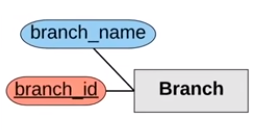
\includegraphics[width=0.6\textwidth]{./Figs/2020-12-24-00-13-51.png}
        % 	\caption{}
        \end{figure}
    
    \item \textbf{The company makes it's money by selling to clients. Each client has a name and unique number to identify it.}
        \begin{figure}[H]
            \centering
            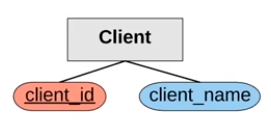
\includegraphics[width=0.6\textwidth]{./Figs/2020-12-24-00-14-18.png}
        % 	\caption{}
        \end{figure}
    
    \item \textbf{The foundation of the company is it's employees. Each employee has a name, birthday, sex, salary and unique number to identify it.}
        \begin{figure}[H]
            \centering
            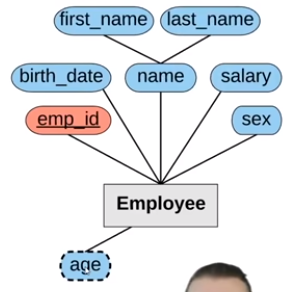
\includegraphics[width=0.6\textwidth]{./Figs/2020-12-24-00-14-53.png}
        % 	\caption{}
        \end{figure}
    
    \item \textbf{An employee can act as a supervisor for other employees at the branch, an employee may also act as the supervisor for employees at other branches. An employee can have at most one supervisor.}
        \begin{itemize}
            \item Notice here the data is defining a relationship.
            \item The relationship is the ``work for''.
            \item All branches must have employees working for them, and all employees must work for a branch. This means a both way total participation.
            \item An employee can work only for ONE branch, and a branch can have multiple employees, hence this is a 1:N cardinality relationship.
        \end{itemize}
        \begin{figure}[H]
            \centering
            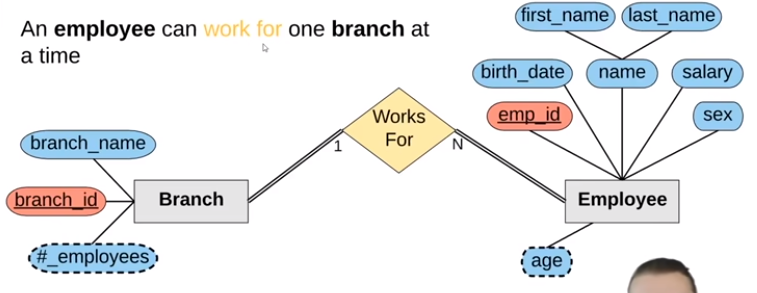
\includegraphics[width=0.6\textwidth]{./Figs/2020-12-24-00-16-07.png}
        % 	\caption{}
        \end{figure}
    
    \item \textbf{An employee can work for one branch at a time, and each branch will be managed by one of the employees that work there. We'll also want to keep track of when the current manager started as manager.}
        \begin{itemize}
            \item Notice the cardinality relationship here, a branch can be managed by one employee and an employee can manage one branch, its 1:1. 
            \item On the ``manages'' relationship we must store the attribute start date, this records when the manager started as manager.
        \end{itemize}
        \begin{figure}[H]
            \centering
            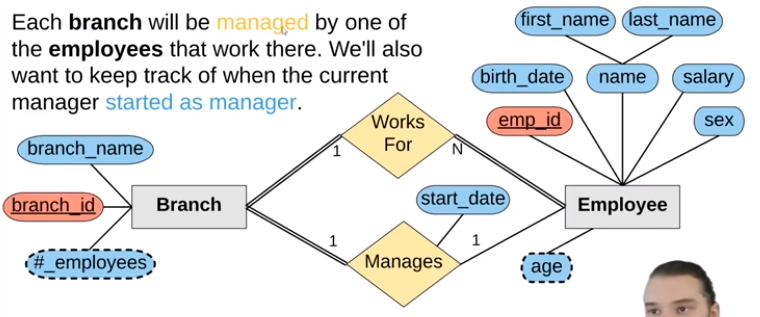
\includegraphics[width=0.6\textwidth]{./Figs/2020-12-24-00-20-01.png}
        % 	\caption{}
        \end{figure}
    
    \item \textbf{An employee can act as a supervisor for other employees at the branch, an employee may also act as the supervisor for employees at other branches. An employee can have at most one supervisor.}
        \begin{itemize}
            \item Here notice that we have a relationship that is with one's self, meaning that an employee can act as a supervisor to other employees, but the supervisor is himself an employee as well.
            \item Lets call the supervisor relationship the ``supervision'' relationship, notice that it is comprised with a supervisor and the supervisee, an employee can have at most one supervisor, and a supervisor can have multiple people to supervise, all the while being an employee also.
            \item The cardinality relationship is thus a 1:N relationship. Because an employee can have at most one supervisor but a supervisor can supervise several employees.
        \end{itemize}
        \begin{figure}[H]
            \centering
            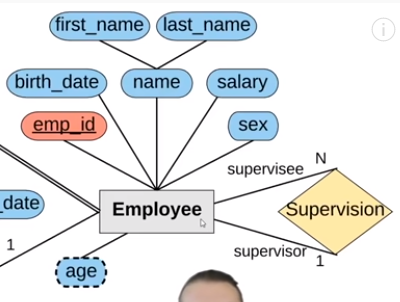
\includegraphics[width=0.6\textwidth]{./Figs/2020-12-24-00-32-14.png}
        % 	\caption{}
        \end{figure}
    
    \item \textbf{A branch may handle a number of clients, with each client having a name and a unique number to identify it. A single client may only be handled by one branch at a time.}
        \begin{itemize}
            \item Now notice the relationship happening between the branch and the client, the client can be handled any number of times by a branch and a single client can only be handled by one branch at a time.
            \item Notice the cardinality relationship, the branch can handle any number of clients but the client can only be handled by only one branch at a time.
            \item Notice that the client has a total participation, because every client needs to be handled by a branch, but the branch has a partial participation because not all branches need to handle every client, in this case it needs to be one branch at a time.
        \end{itemize}
        \begin{figure}[H]
            \centering
            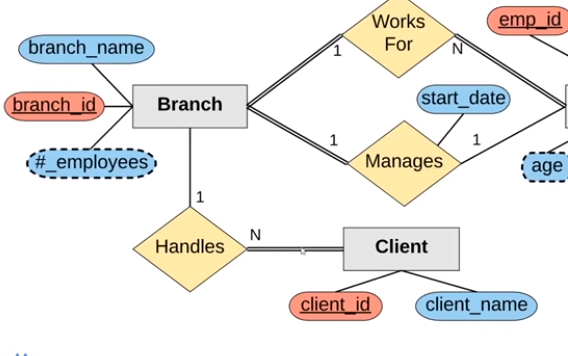
\includegraphics[width=0.6\textwidth]{./Figs/2020-12-24-00-38-06.png}
        % 	\caption{}
        \end{figure}
    
    \item \textbf{Employees can work with clients controlled by their branch to sell them stuff. If necesary, multiple employees can work with the same client. We'll want oto keep track of how many dollars worth of stuff each employee sells to each client they work with.}
        \begin{itemize}
            \item Notice the cardinality, employees can work with clients, any number of clients and clients can have any number of employees working with them, It's an N:M cardinality relationship.
            \item Notice here the relationship is the client and the employee ``working'' together, or ``works with''. When this relationship takes place a sale may take place, this is a relationship attribute ``sales''.
            \item Notice the participation, all clients must work with and interact with employees but not all employees must work with clients.
        \end{itemize}
        \begin{figure}[H]
            \centering
            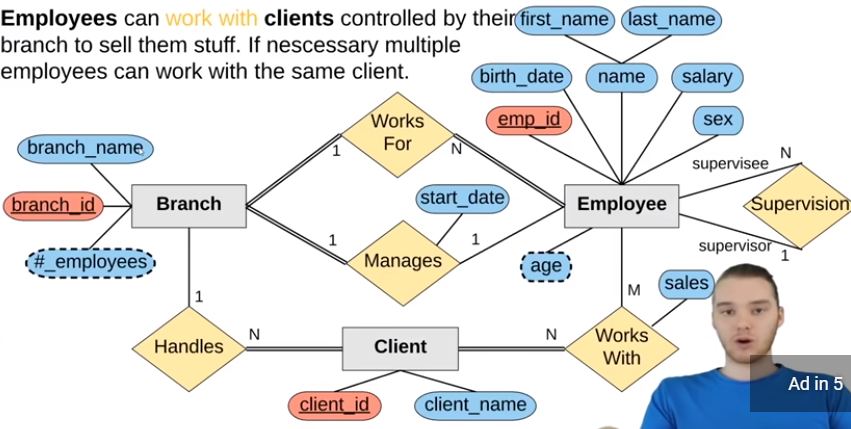
\includegraphics[width=0.6\textwidth]{./Figs/2020-12-24-00-39-58.png}
        % 	\caption{}
        \end{figure}

    \item \textbf{Many branches will need to work with suppliers to buy inventory. For each supplier we'll keep track of their name and the type of product they're selling the branch. A single suppler may supply products to multiple branches.}
        \begin{itemize}
            \item This is a case where we would need to define a weak entity and weak relationship.
            \item Notice the branch supplier supplies a specific branch or branches, we also want to keep track of which supplier is supplying with branch. Do this using the weak relationship ``supplies''.
            \item Notice that there can be any number of suppliers per branch and any branches per supplier. The cardinality relationship is N:M.
            \item Notice the participation, as always weak entities have total participation in the relationship and the string entity haves in this case partial participation, because not all branches must be supplied. 
        \end{itemize}
        \begin{figure}[H]
            \centering
            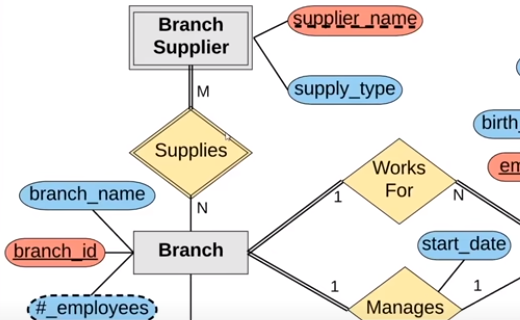
\includegraphics[width=0.6\textwidth]{./Figs/2020-12-24-00-48-35.png}
        % 	\caption{}
        \end{figure}
    
    \item The whole diagram looks like this:
        \begin{figure}[H]
            \centering
            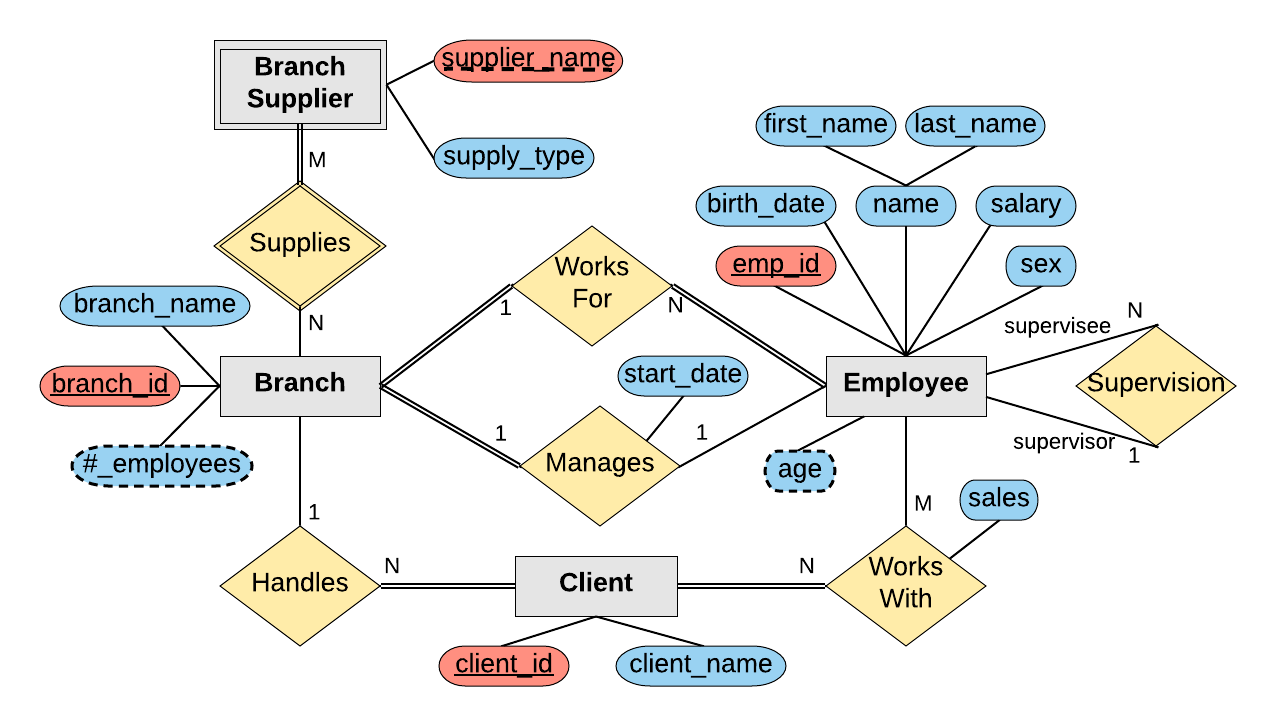
\includegraphics[width=0.6\textwidth]{./Figs/2020-12-24-20-14-44.png}
        % 	\caption{}
        \end{figure}
\end{itemize}
